%%%%%%%%%%%%%%%%%%%%%%%%%%%%%%%%%%%%%%
% LaTeX poster template
% Created by Nathaniel Johnston
% August 2009
% http://www.nathanieljohnston.com/2009/08/latex-poster-template/
%%%%%%%%%%%%%%%%%%%%%%%%%%%%%%%%%%%%%%

\documentclass[final, table]{beamer}
%\usepackage[scale=1.24]{beamerposter}
\usepackage[size=a1,scale=1.1]{beamerposter}
\usepackage{graphicx}			% allows us to import images
\usepackage{subfigure}

%-----------------------------------------------------------
% Define the column width and poster size
% To set effective sepwid, onecolwid and twocolwid values, first choose how many columns you want and how much separation you want between columns
% The separation I chose is 0.024 and I want 4 columns
% Then set onecolwid to be (1-(4+1)*0.024)/4 = 0.22
% Set twocolwid to be 2*onecolwid + sepwid = 0.464
%-----------------------------------------------------------

\newlength{\sepwid}
\newlength{\onecolwid}
\newlength{\twocolwid}
\newlength{\threecolwid}
\setlength{\paperwidth}{48in}
\setlength{\paperheight}{36in}
%\setlength{\paperwidth}{42in}
%\setlength{\paperheight}{36in}
\setlength{\sepwid}{0.024\paperwidth}
\setlength{\onecolwid}{0.22\paperwidth}  % For 4 columns
%\setlength{\onecolwid}{0.30\paperwidth}   % 3 columns
\setlength{\twocolwid}{0.464\paperwidth}
\setlength{\threecolwid}{0.708\paperwidth}
\setlength{\topmargin}{-0.5in}
\usetheme{confposter}
\usepackage{exscale}
\usepackage[font=singlespacing]{caption}
\usepackage{multirow}

%-----------------------------------------------------------
% The next part fixes a problem with figure numbering. Thanks Nishan!
% When including a figure in your poster, be sure that the commands are typed in the following order:
% \begin{figure}
% \includegraphics[...]{...}
% \caption{...}
% \end{figure}
% That is, put the \caption after the \includegraphics
%-----------------------------------------------------------

%\usecaptiontemplate{
%\small
%\structure{\insertcaptionname~\insertcaptionnumber:}
%\insertcaption}
\setbeamertemplate{caption}[numbered]

%-----------------------------------------------------------
% Define colours (see beamerthemeconfposter.sty to change these colour definitions)
%-----------------------------------------------------------

\setbeamercolor{block title}{fg=dblue,bg=white}
\setbeamercolor{block body}{fg=black,bg=white}
\setbeamercolor{block alerted title}{fg=white,bg=dblue!70}
\setbeamercolor{block alerted body}{fg=black,bg=dblue!10}

%-----------------------------------------------------------
% Math commands
%-----------------------------------------------------------
\newcommand{\X}{\mathcal{X}}
\newcommand{\Y}{\mathcal{Y}}
\newcommand{\G}{\mathcal{G}}
\newcommand{\norm}[1]{\left | \left | #1 \right | \right |}
\newcommand{\reals}{\mathbb{R}}
\newcommand{\scrF}{\mathcal{F}}
\newcommand{\E}{\mathbb{E}}
\newcommand{\K}{\mathcal{K}}
\newcommand{\PP}{\mathbb{P}}
\newcommand{\N}{\mathbb{N}}
\newcommand{\Dir}{\text{Dir}}
\newcommand{\DP}{\text{DP}}
\newcommand{\Pois}{\text{Pois}}
\newcommand{\BP}{\text{BP}}
\newcommand{\BeP}{\text{BeP}}
\newcommand{\borel}{\mathcal{B}}
\newcommand{\Beta}{\text{Beta}}
\newcommand{\Discrete}{\text{Discrete}}
\newcommand{\Ber}{\text{Bernoulli}}
\newcommand{\CRP}{\text{CRP}}
\newcommand{\IBP}{\text{IBP}}
\newcommand{\Norm}{\text{N}}
\newcommand{\B}{\mathcal{B}}
\newcommand{\Corr}{\text{Corr}}
\newcommand{\Un}{\text{Un}}
\newcommand{\CRM}{\text{CRM}}
\newcommand{\NiG}{\text{NiG}}
\newcommand{\Cat}{\text{Cat}}
\newcommand{\T}{\mathcal{T}}
\newcommand{\Ga}{\text{Ga}}
\newcommand{\notrightarrow}{\centernot\rightarrow}
\newcommand{\gap}{\text{    }}



%-----------------------------------------------------------
% Name and authors of poster/paper/research
%-----------------------------------------------------------

\title{Probabilistic Synapse Detectionin Array Tomography}
\author{
Anish K. Simhal		\textsuperscript{1*},
Cecilia Aguerrebere		\textsuperscript{1},
Forrest Collman		\textsuperscript{2}
Joshua T. Vogelstein		\textsuperscript{3},
Kristina D. Micheva		\textsuperscript{4}, \\
Richard J. Weinberg		\textsuperscript{5},
Stephen J. Smith		\textsuperscript{2},
Guillermo Sapiro		\textsuperscript{1, 6}}
\institute{\textsuperscript{1}Electrical and Computer Engineering, Duke University 
\textsuperscript{2} Synapse Biology, Allen Institute for Brain Sciences 
\textsuperscript{3} Department of Biomedical Engineering, Johns Hopkins University
\textsuperscript{4} Molecular and Cellular Physiology, Stanford University School of Medicine
\textsuperscript{5} Department of Cell Biology and Physiology, University of North Carolina
\textsuperscript{6} Department of Biomedical Engineering, Department of Computer Science, Department of Mathematics, Duke University}

%-----------------------------------------------------------
% Start the poster itself
%-----------------------------------------------------------
\begin{document} 
\addtobeamertemplate{headline}{} 
{\begin{tikzpicture}[remember picture, overlay]
\node [anchor=north west, inner sep=3cm]  at (current page.north west)
{
\includegraphics[scale=0.225]{figs/duke_univ_blue}};
\end{tikzpicture}
\vspace{6cm} %twiddle with this later...
\begin{tikzpicture}[remember picture, overlay]
\node [anchor=north east, inner sep=3cm]  at (current page.north east)
{
\includegraphics[scale=0.55]{figs/IID_logo}};
\end{tikzpicture}
}
\begin{frame}[t]  
\begin{columns}[t]  % align column content at top

% First column
\begin{column}{\sepwid}\end{column}  % spacer column
\begin{column}{\onecolwid} 

\begin{block}{Challenge} 
\begin{itemize} 
\item Unsupervised automatic detection of specific synaptic subtypes with confidence values using array tomography data
\end{itemize} 

%\textbf{{}}

\begin{figure}
\centering
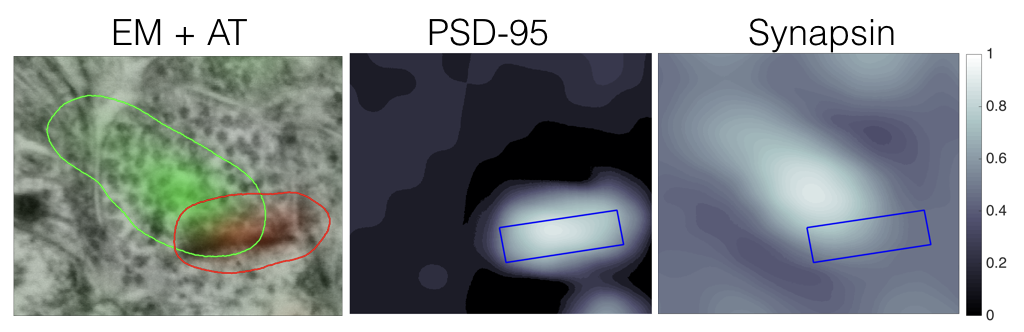
\includegraphics[width=1\textwidth]{figs/em_if_outlines}
\caption{Left: PSD-95 (red) and Synapsin (green) data overlaid on EM data.  Center: PSD-95 IF image. Right: Synapsin IF image. Synaptic cleft marked in blue.}
\label{fig:synapseOverview}
\end{figure}

\end{block}

\begin{block}{Background} 
\begin{itemize} 
\item \textbf{What is a Synapse?}
\end{itemize} 
\begin{figure}
\centering
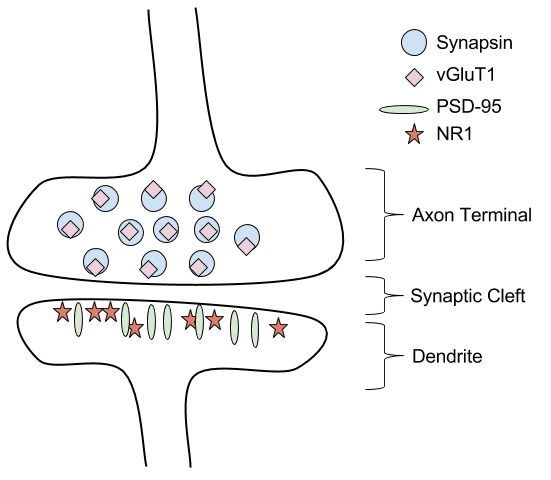
\includegraphics[width=0.6\textwidth]{figs/Chemical_Synapse}
\caption{Molecular architecture of a excitatory PSD-95 expressing synapse depicted in a simplified cartoon form}
\label{fig:Chemical_Synapse}
\end{figure}

\begin{itemize} 
\item \textbf{Array Tomography (AT) Pipeline}
\end{itemize} 

\begin{figure}
\centering
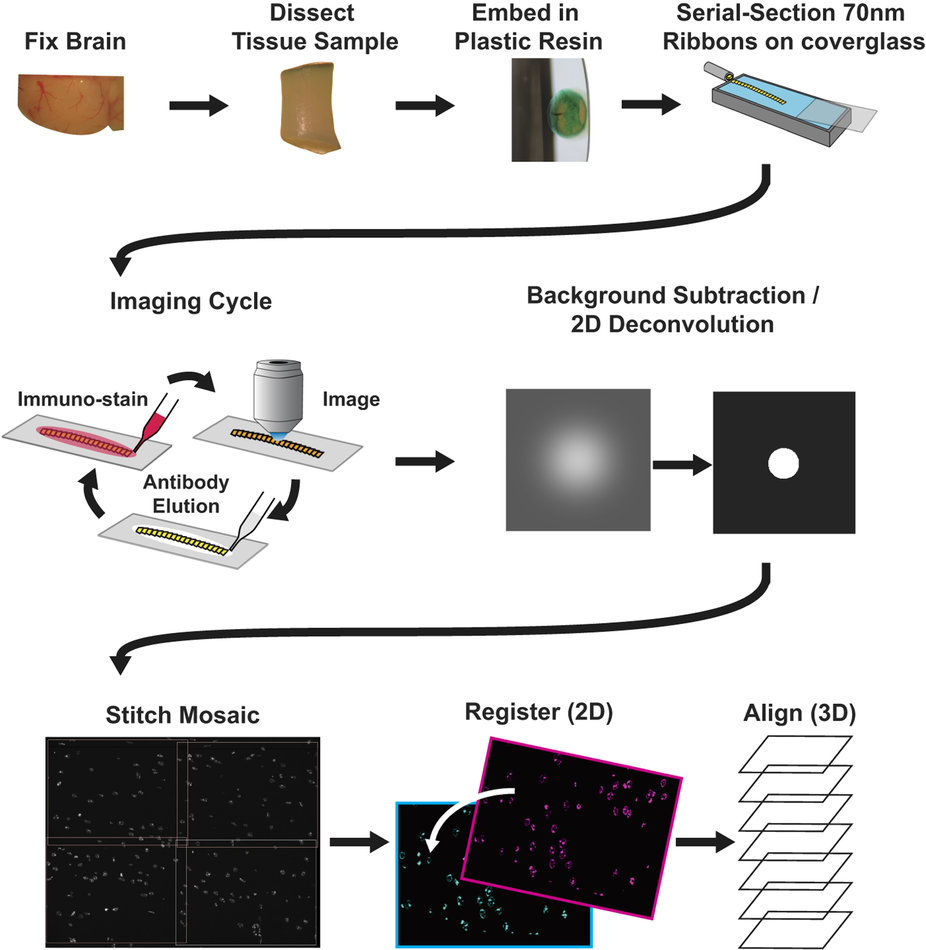
\includegraphics[width=0.75\textwidth]{figs/at_diagram3}
\caption{Array Tomography Methodology  \cite{Weiler}}
\end{figure}


\end{block} 


\end{column}

% Second column
\begin{column}{\sepwid}\end{column}  % spacer column
\begin{column}{\twocolwid}



\begin{block}{Action}

\begin{columns}[t]  % align column content at top

\begin{column}{\onecolwid}

\begin{itemize} 
\item \textbf{Overview of Proposed Method}
\end{itemize} 


\begin{figure}
\centering
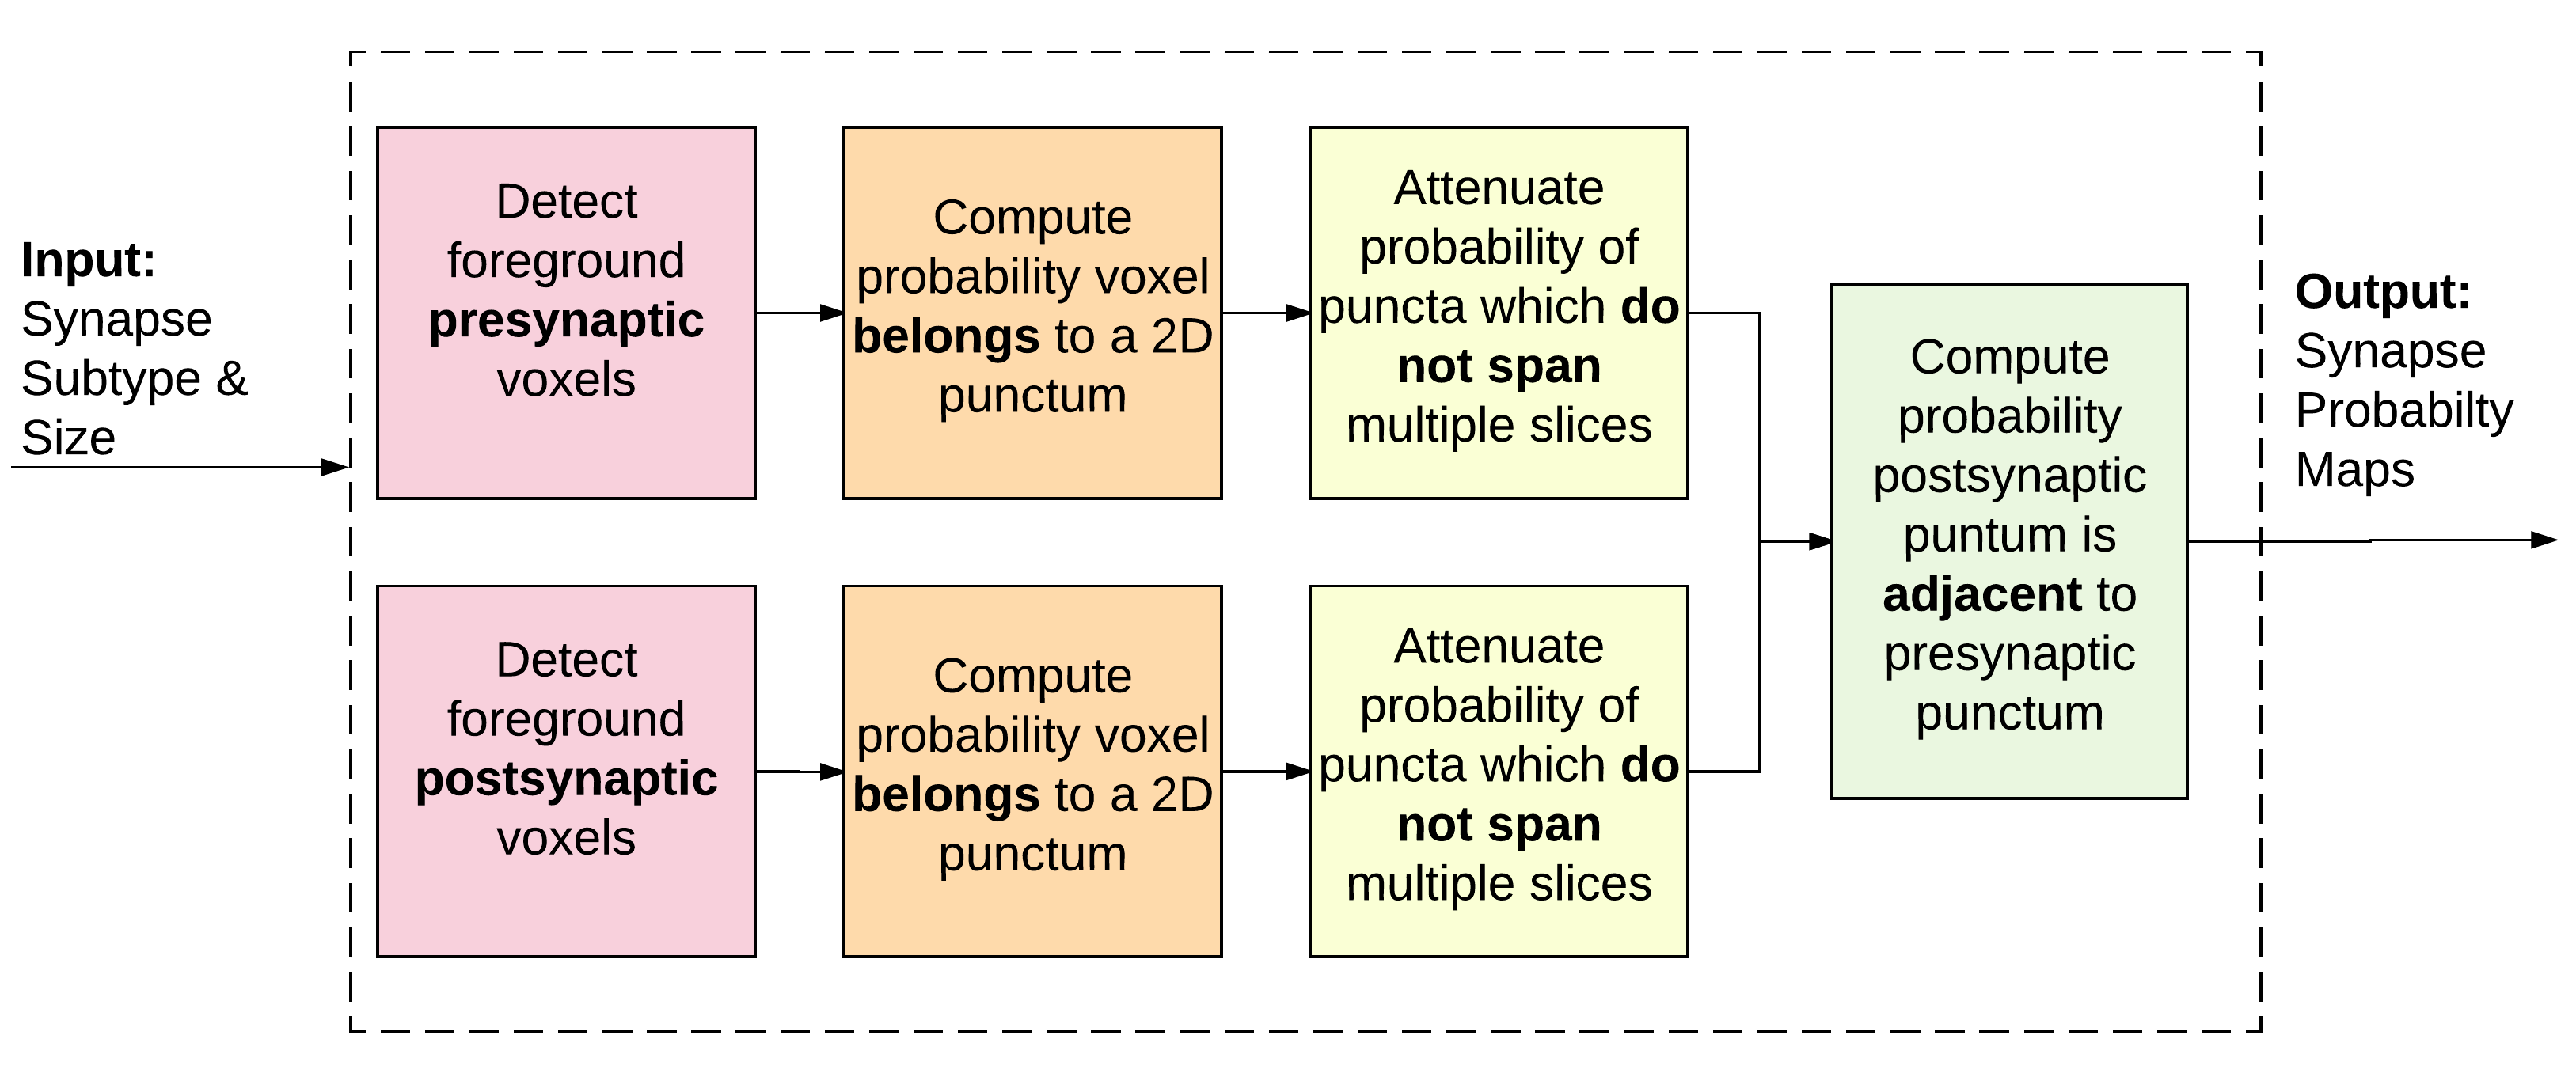
\includegraphics[width=1\textwidth]{figs/pipeline2}
\label{fig:pipeline}
\end{figure}

\begin{itemize} 
\item \textbf{Step 1: Foreground Probability} %Model background $p_B$ from the raw data. Foreground probability is one minus the background. 
\end{itemize} 

\begin{equation} 
p_B(x,y,z) = \frac{1}{\sigma_B \sqrt{2 \pi}} \int^{\infty}_{v(x,y,z)} e^{\frac{-(t - \mu_B)^2}{2 \sigma_B^2}} d t.
\end{equation} 

\begin{equation}
p_F(x,y,z) = 1 - p_B(x,y,z).
\end{equation}

\begin{figure}
\centering
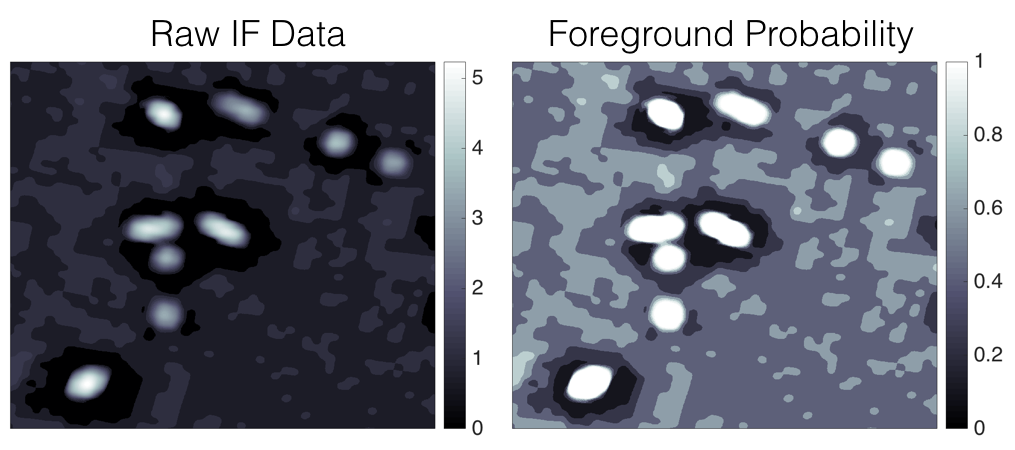
\includegraphics[width=1\textwidth]{figs/lograw_prob}
\caption{(Left) Logarithm of the IF raw data. (Right) Foreground probability map.  Slices of the PSD-95 antibody of size $5.268 \times 5.827$ $\mu m$.}
\label{fig:raw_prob} 
\end{figure}


% (Left) Logarithm of the IF raw data. (Right) Foreground probability map.  Slices of the PSD-95 antibody of size $5.268 \times 5.827 \mu m$.

%Cutout of size $5.268 \times 5.827 \mu m$ of the logarithm of the IF raw data (left) and the corresponding image of the foreground probability map (right) of one slice of the PSD-95 antibody.

\begin{itemize} 
\item \textbf{Step 2: 2D Puncta Probability.}  %Output is probability a voxel belongs to a group of high probability voxels. 
\end{itemize} 


\begin{align} 
p_P(x, y, z) = \prod_{i=x-W}^{x+W} \prod_{j=y-W}^{y+W} p_F(i,j, z),
\end{align} 
$W$ is the expected size of a punctum.  % where, $p_F$ is the foreground probability and
\begin{figure}[!h]
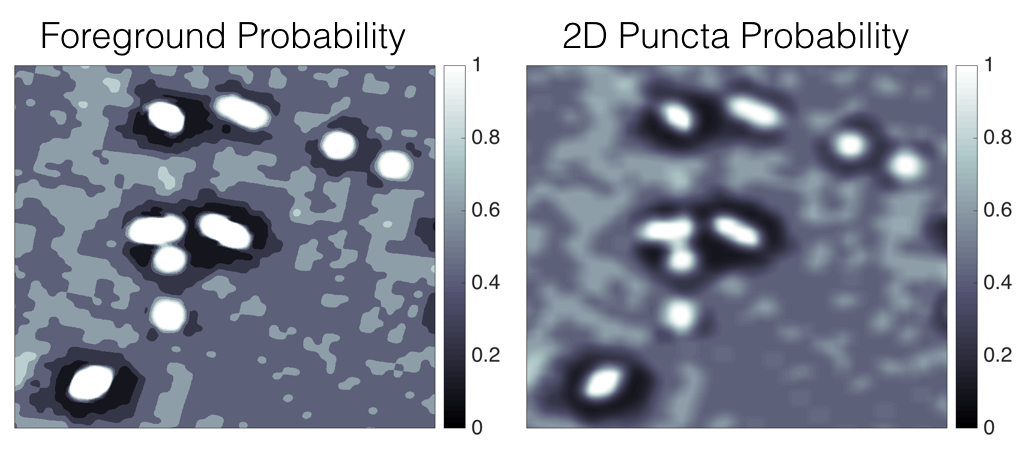
\includegraphics[width=1\textwidth]{figs/prob_conv}
\caption{(Left) Probability map. (Right) Probability map of each pixel belonging to a 2D punctum.}
\label{fig:prob_conv}
\end{figure}


\end{column}

% Third column

\begin{column}{\sepwid}\end{column}  % spacer column
\begin{column}{\onecolwid}
%\begin{block}{Action} 
\begin{itemize} 
\item \textbf{Step 3: 3D Puncta Probability} %Punctum which do not span multiple slices are down weighted by a factor, $f(x, y, z)$ 
\end{itemize} 

\begin{equation} 
f(x, y, z) = \exp \left \{- \sum_{j=j_{start}}^{j=j_{end}} [p_P(x, y, z) - p_P(x, y, z+j)]^2 \right \}
\label{eq:factor}
\end{equation} 

\begin{equation}
p_{3DP}(x,y,z)= p_P(x,y,z) f(x,y,z),
\label{eq:p3dp} 
\end{equation}
\vspace{1cm}

\begin{figure}
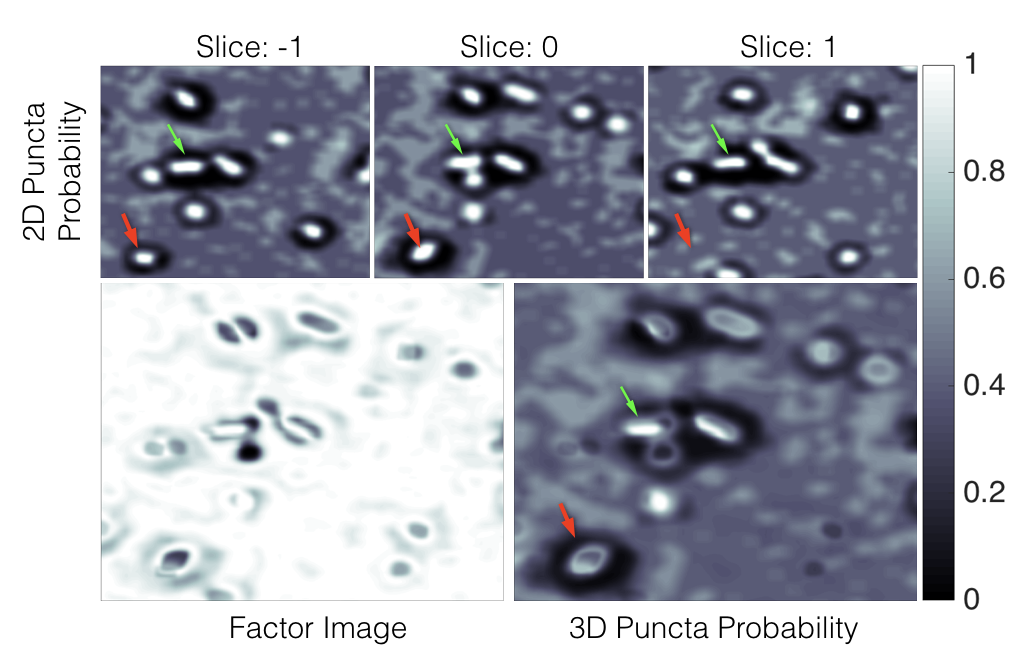
\includegraphics[width=1\textwidth]{figs/factor_result}
\caption{\textbf{Top:} Three consecutive slices of the 2D puncta probability. \textbf{Bottom:} Factor image given by Eq.~\eqref{eq:factor} (left) and the corresponding 3D puncta probability (right) of the center slice in the top row. Each image is a cutout of size $2261 \times 2501$ pixels or $5.268 \times 5.827 \mu m$.}
\label{fig:factor_result}
\end{figure}

\vspace{1cm}
\begin{itemize} 
\item \textbf{Step 4: Presynaptic and Postsynaptic Puncta Adjacency}.  %For the final output, multiply the postsynaptic probability by the maximum presynaptic probability value in an adjacent region. 
\end{itemize} 

\begin{figure}[!h]
\centering
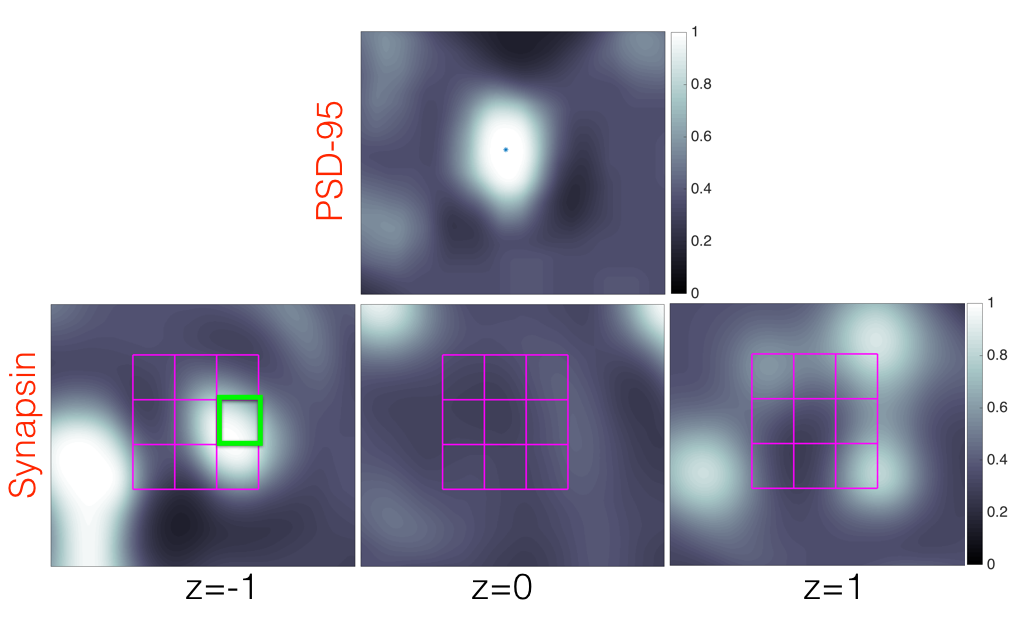
\includegraphics[width=1\textwidth]{figs/gridsearch}
\caption{\textbf{First row:} cutout of PSD-95 Punctum with center pixel highlighted. \textbf{Second row:} synapsin cutouts with the search grid overlaid.} 
\end{figure} 


\end{column}
\end{columns} 
\end{block}
\end{column} 

% Fourth column
\begin{column}{\sepwid}\end{column}  % spacer column
\begin{column}{\onecolwid}



\begin{block}{Resolution} 
\begin{itemize} 
\item \textbf{Result:} 
\end{itemize}  

\begin{figure}[!h]
\centering
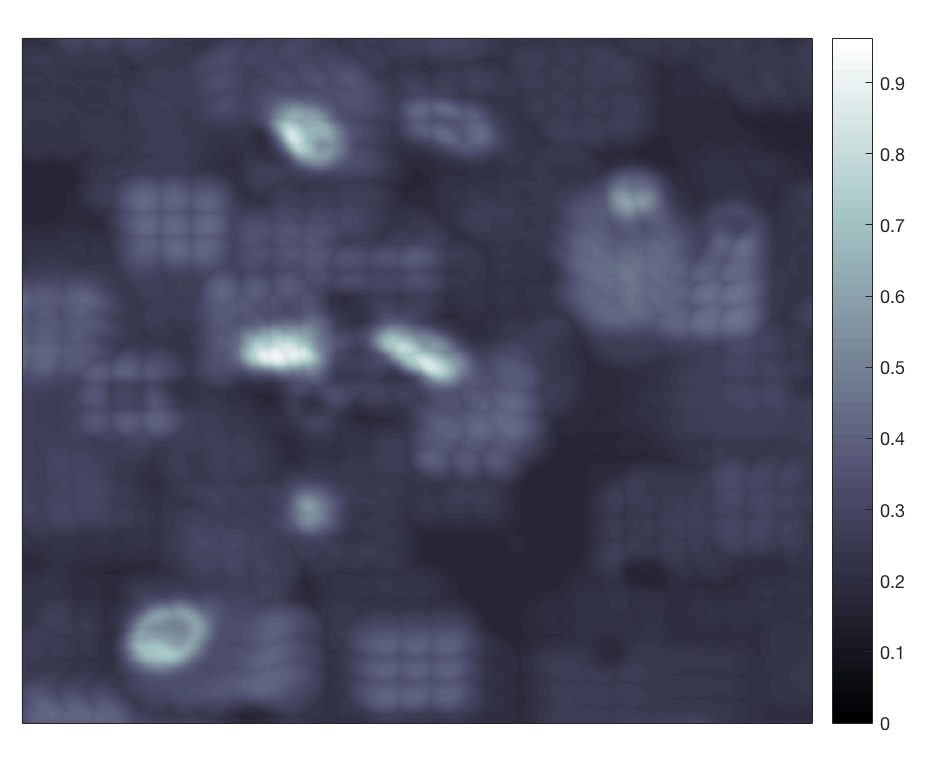
\includegraphics[width=0.6\textwidth]{figs/silane_output}
\caption{Output probability map, each pixel's intensity value represents to the probability of it belonging to a synapse. }
\end{figure}



\begin{figure}[!h]
\centering
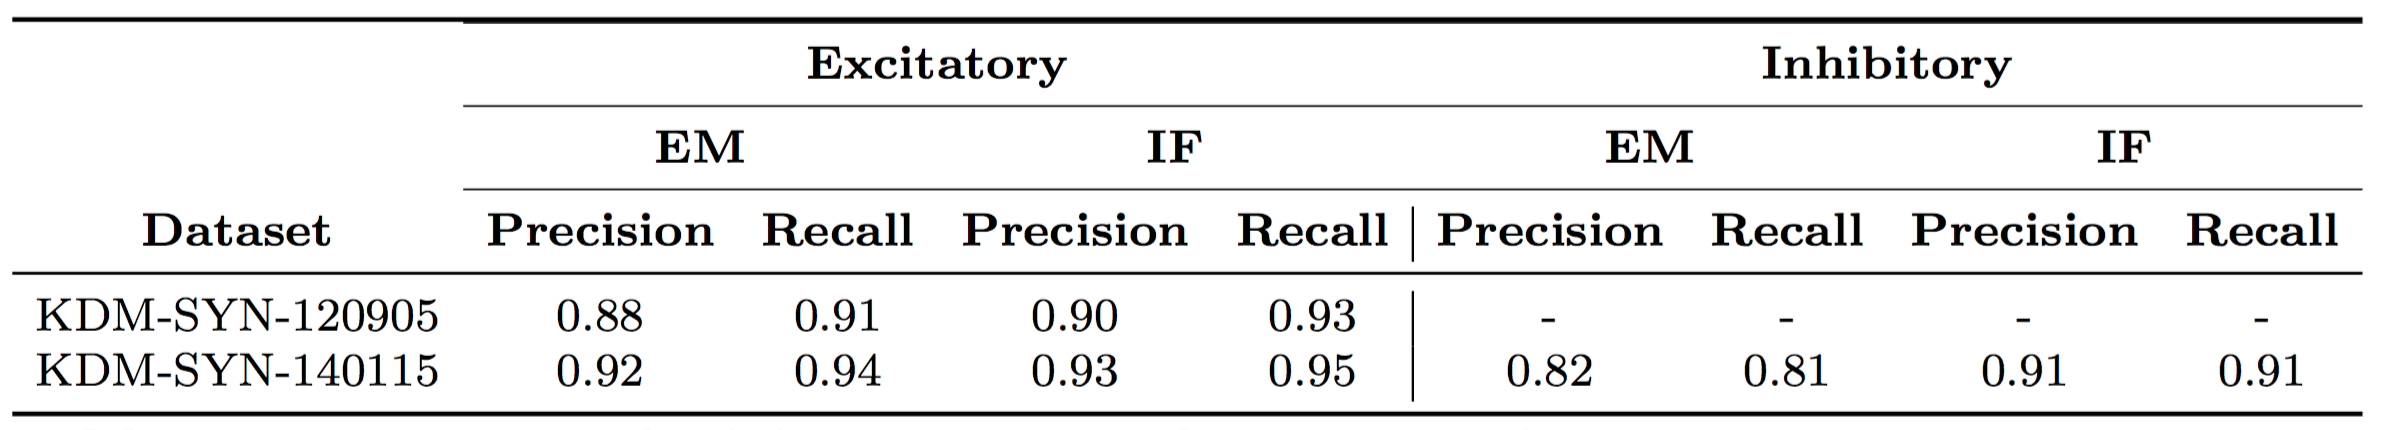
\includegraphics[width=1\textwidth]{figs/table1}
\caption{Precision and recall values on conjugate array tomography data}
\label{fig:pr_curves}
\end{figure}


\begin{figure}[!h]
\centering
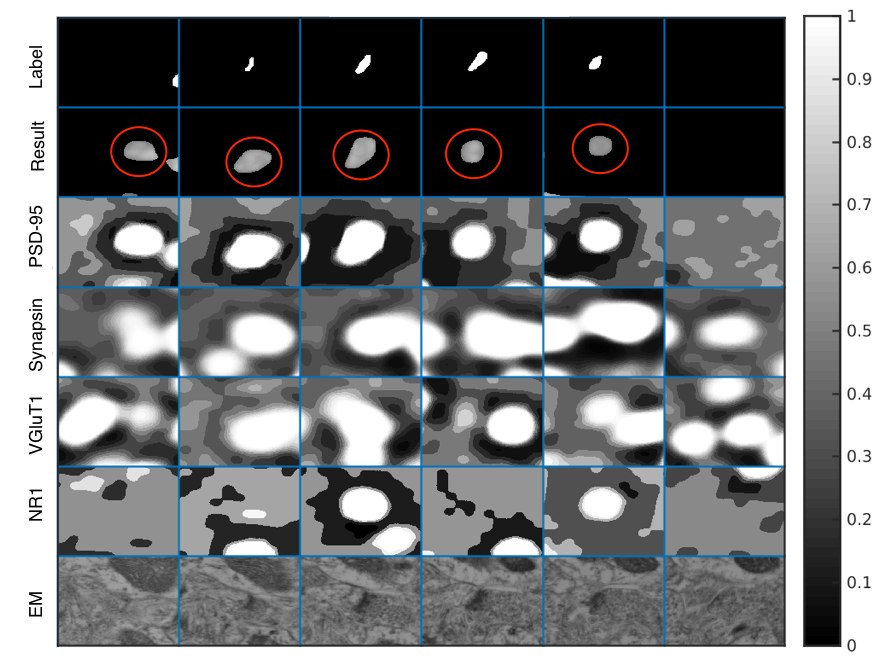
\includegraphics[width=0.8\textwidth]{figs/synaptogramSilane}
\caption{Synaptogram showing IF data for an EM identified synapse.  Each `block' is $1.221 \mu m \times 1.233 \mu m$. }
\label{fig:synaptogramSilane}
\end{figure}






\end{block} 

\begin{block}{Acknowledgments} 

\tiny{This work was supported by the National Institutes of Health (NIH-TRA 1R01NS092474), the Allen Institute for Brain Sciences (AIBS), the U.S. Office of Naval Research (ONR), the U.S. Army Research Office (ARO), the National Science Foundation (NSF), and the U.S. National Geospatial Intelligence Agency (NGA).}
\end{block} 


\vspace{-0.05in}
\begin{block}{References}
\tiny{
\begin{thebibliography}{99}
\bibitem{Busse}
Busse B, Smith S. Automated analysis of a diverse synapse population. PLoS Comput Biol. 2013 Mar 28;9(3):e1002976.

\bibitem{Collman} 
Collman F, Buchanan J, Phend KD, Micheva KD, Weinberg RJ, Smith SJ. Mapping synapses by conjugate light-electron array tomography. The Journal of Neuroscience. 2015 Apr 8;35(14):5792-807.
 
\bibitem{Harris} 
Harris KM, Weinberg RJ. Ultrastructure of synapses in the mammalian brain. Cold Spring Harbor Perspectives in Biology. 2012 May 1;4(5):a005587.

\bibitem{Micheva2} 
Micheva KD, Smith SJ. Array tomography: a new tool for imaging the molecular architecture and ultrastructure of neural circuits. Neuron. 2007 Jul 5;55(1):25-36.

\bibitem{Micheva1} 
Micheva KD, Busse B, Weiler NC, O'Rourke N, Smith SJ. Single-synapse analysis of a diverse synapse population: proteomic imaging methods and markers. Neuron. 2010 Nov 18;68(4):639-53.


\bibitem{Weiler} 
Weiler NC, Collman F, Vogelstein JT, Burns R, Smith SJ. Synaptic molecular imaging in spared and deprived columns of mouse barrel cortex with array tomography. Scientific Data. 2014 Dec 23;1.

\end{thebibliography}}
\end{block}

\end{column}


\end{columns}
\end{frame}
\end{document}
